\section{Teknologier}
\label{sec:teknologier}
Systemet er en webapplikation, hvor der er lagt vægt på enkelt og forståeligt design, effektivitet, fleksibilitet og brugbarhed. For at kunne opfylde alle disse krav og kriterier, som er beskrevet i \secref{sec:kriterier}, har vi gjort brug af nogle forskellige webudviklings- og programmeringsteknologier.

Vi har brugt følgende teknologier:

\begin{itemize}[noitemsep]
\item HTML og CSS
\item MySQL %og phpMyAdmin
\item JavaScript, jQuery, jQuery UI, AJAX og JSON
\item Ruby on Rails
\end{itemize}

Vi har brugt HTML\cite{htmlwiki} til at designe brugergrænsefladen af hjemmesiden med. HTML fungerer godt til opmærkning og strukturering af hjemmesider, men ren HTML er ikke særlig flot at se på. For at designe hjemmesiden har vi brugt CSS\cite{csswiki}, der er et sprog, som bruges til at beskrive, hvordan man ønsker indholdet af bl.a. et HTML-dokument skal præsenteres i \fx en webbrowser.

Hvad angår databaser, så har vi har brugt MySQL\cite{mysqlwiki}, der er en flertrådet SQL-databaseserver, som understøtter flere samtidige brugere. %I og med at vi består af en gruppe af individer med vidt forskellige kompetencer og erfaringer med web- og systemudvikling, har vi brugt det browserbaserede program, phpMyAdmin\cite{phpmyadmin}, til at administrere og opdatere MySQL-databasen på en mere brugervenlig måde. phpMyAdmin præsenterer en letforståelig brugergrænseflade til redigering af databasen. Udviklerne bag MySQL har også udviklet deres eget administrationsmodul til databasen, men den skal installeres på en computer, hvorimod phpMyAdmin køres på serveren med databasen, der præsenteres direkte via webbrowseren, hvilket betyder, at vi ikke behøver installere et program på seks forskellige computere, men blot kan bruge det samme interface via webbrowseren.

For at gøre hjemmesiden dynamisk og brugervenlig, bruger vi JavaScript\cite{javascriptwiki}, som er et objektorienteret scriptsprog, som de fleste moderne webbrowsere forstår. Derudover har vi også brugt jQuery\cite{jquery} sammen med JavaScript. jQuery er et programbibliotek, der bygger oven på JavaScript. Det forøger kraftigt funktionalitet af JavaScript og samtidig formindsker antallet af linjer i filerne, da jQuery-objekter indeholder mange metoder. AJAX\cite{ajaxwiki} og JSON\cite{jsonwiki} bliver ydereligere brugt til at gøre webapplikationen asynkront. Vi udnytter forskellige widgets og animationer inkluderet i jQuery UI\cite{jqueryuiwiki} med et eksisterende tema. jQuery UI bygger oven på jQuery og tilbyder yderligere funktionalitet i forbindelse med designet af webapplikationer. Figur \ref{fig:toolbar} illustrerer tre forskellige jQuery UI ``widgets'', som brugeren kommer i kontakt med, når der bliver udført en søgning på foodl-hjemmesiden. AJAX gør det muligt at udveksle data mellem hjemmeside og server uden at siden skal gennemgå en fuld sideopdatering hver gang, der sker en dataoverførsel, for at vise det nye indhold. Hovedsageligt sker alle dataoverførsler i baggrunden og brugeren præsenteres med disse ændringer med det samme. \Fx bliver søgeresultatsiden opdateret dynamisk, når man ændrer i sorteringen. AJAX står for ``Asynchrounous JavaScript and XML'', og navnet antyder at XML bruges til udvekslingen af oplysninger fra serveren til klienten (webbrowseren). Nu om dage anvendes JSON dog som regel som erstatning for XML i forbindelse med AJAX. JSON er et simpelt dataudvekslingsformat som bygger på JavaScript-syntax, og understøtter de simple JavaScript typer, såsom tal, tekststrenge, arrays og objekter. Det gør det ideelt til \fx at sende et objekt eller et array af objekter fra serveren til klienten.

\begin{figure}[H]
\centering

\includegraphics[scale=0.6]{billeder/jqueryuieksempel.png}
\capt{Figuren viser tre forskellige eksempler på widgets, der er lavet vha. jQuery UI. Til venstre ses en samling af tre knapper, som fungerer som afkrydsningsbokse, hvilket betyder, at man kan markere flere af gangen. Disse knapper gør det muligt for brugeren at begrænse søgeresultatet efter disse tre kriterier for tilberedningstiden. Midt for ses en justerbar knap, der gør det muligt for brugeren at skalere opskrifterne. Til højre ses endnu en samling af tre knapper, der fungerer som radioknapper, hvilket betyder, at man kun kan vælge én knap af gangen. Disse knapper giver brugeren mulighed for at sortere resultaterne efter navn, relevans eller tilberedningstid.}
\label{fig:toolbar}
\end{figure}

Derudover har vi anvendt Ruby on Rails \cite{rubyonrailswiki}, der er et webudviklingsframework bygget oven på programmeringssproget Ruby, til at lave webapplikationer. Intentionerne bag Rails var at skabe et framework, der gjorde det lettere og hurtigere for webudviklere at udvikle webapplikationer, hvilket også er en af de væsentlige årsager til, at vi vælger at anvende Rails. 

Målet med Rails blev bl.a. opnået vha. af følgende filosofi:
\begin{quote}
``konventioner over konfigurationer''
\end{quote} 

Filosofien har både sine fordele og ulemper. Det er en ulempe, at webudvikleren skal have arbejdet meget med Rails i forvejen, for at kunne huske de mange konventionerne og kommandoer, eller bruge en masse tid på at slå dem op, når de skal bruges. Det er på den anden siden en fordel, at webudviklere, vha. Rails' konventioner, kan lave applikationer, som kan udrette meget, ud fra få linjers kode. Det gør det også lettere at kigge på andre, eksisterende Rails-applikationer uden, at man bliver nødt til at sætte sig ind i et hav af konfigurationsfiler. Rails viser allerede fra første møde, at der skal meget lidt arbejde til, for at få et stort afkast. 

\begin{figure}
	\centering
	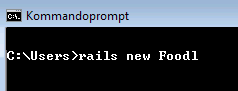
\includegraphics[scale=0.6]{billeder/Rails-new-foodl.png}
	\capt{Railskommando, der indtastes i kommandopromten, hvorefter rails genererer en mappe med en fuldtfungerende web-applikation, kaldet ``Foodl''}
	\label{fig:Rails-new-foodl}
\end{figure}

Enhver Railsapplikation tager udgangspunkt i arkitekturen Model-View-Controllerarkitektur. Mappen med webapplikationen består af en lang række undermapper, hvori ``models'', ``views'' og ``controllers'' bl.a. befinder sig. Kort sagt genererer Rails, vha. \texttt{new}-kommandoen, hele skelettet for webapplikationen, og derefter er det ``bare'' at fylde det indhold, man ønsker i sin webapplikation, i de rigtige mapper. Denne Model-View-Controllerarkitektur er forklaret på en overordnet plan i \secref{subsec:mvc}.
